\documentclass[12pt]{article}
\usepackage{amsmath}
\usepackage{hyperref}
\usepackage[latin1]{inputenc}
\usepackage{graphicx}


\title{Zadanie 9}
\author{Wojciech Ganobis}
\date{26/03/20}

\begin{document}

\begin{description}
  \item[a)]
  
 Niech $X \sim U [-2, 2]$

\begin{figure}[h]
	\centering
   
		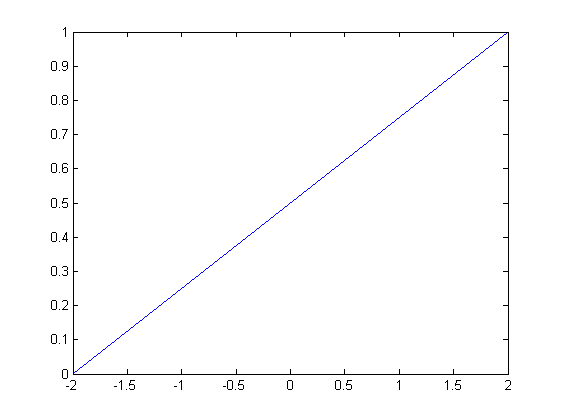
\includegraphics[width=8cm]{aX}
		\caption{X}
\end{figure}

  $Y = \|X\|$
  $$F(y) = P(Y \leq y) = P(\|X\| \leq y) = P(-y \leq X \leq y) = P(X \leq y) - P(X \leq -y)$$
  $$F_{Y} = F_{X}(y) - F_{X}(-y)$$
  
  $Y \sim U[0, 2]$
\begin{figure}[h]
	\centering
   
		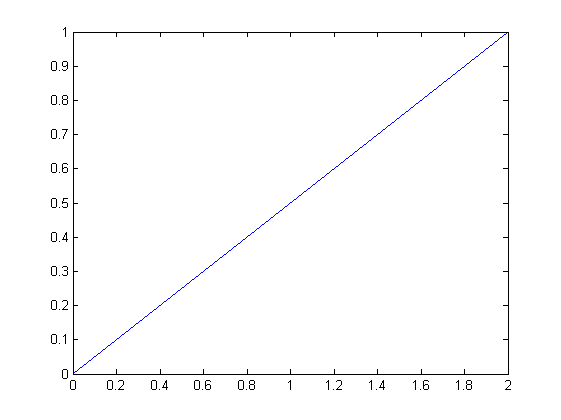
\includegraphics[width=8cm]{aY}
		\caption{Y}
\end{figure}
  
  \item[b)] 
  
   Niech $X \sim U [-1, 1]$\\

   \begin{figure}[h]
	\centering
   
		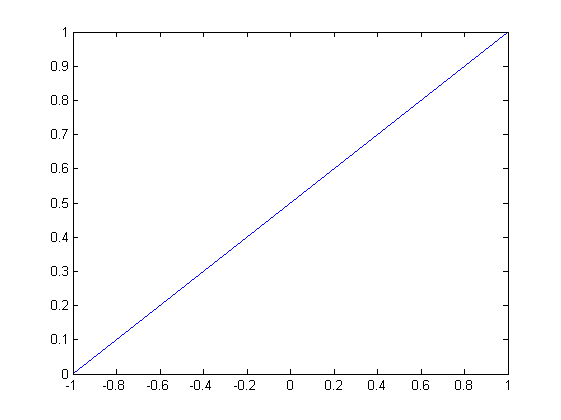
\includegraphics[width=8cm]{bX}\\
		\caption{X}
\end{figure}
   \begin {itemize}
   
   \item 

   $Y = X^{3}$
   $$F(y) = P(Y \leq y) = P(X^{3} \leq y) = P(X \leq \sqrt[3]{y})$$
   $$F_{Y} = F_{X}(\sqrt[3]{y})$$

\begin{figure}[h]
	\centering
   
		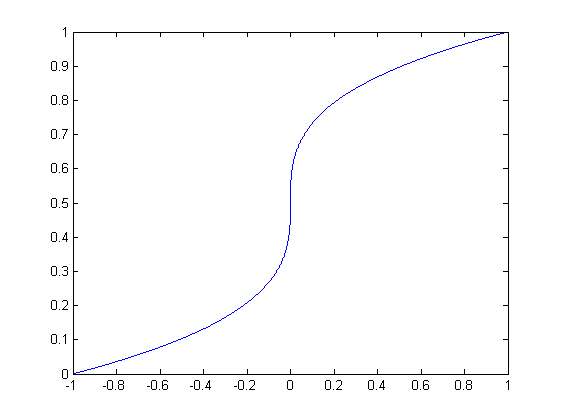
\includegraphics[width=8cm]{bY}
		\caption{Y}
\end{figure}
   
   \item
   
   $Z = X^{2}$
   $$F(y) = P(Z \leq y) = P(X^{2} \leq y) = P(-\sqrt{y} \leq X \leq \sqrt{y}$$
   $$P(X \leq \sqrt{y}) - P(X \leq -\sqrt{y})$$
   $$F_{Z} = P(x \leq \sqrt{y}) - P(X \leq -\sqrt{y})$$
     \begin{figure}[h]
	\centering
   
		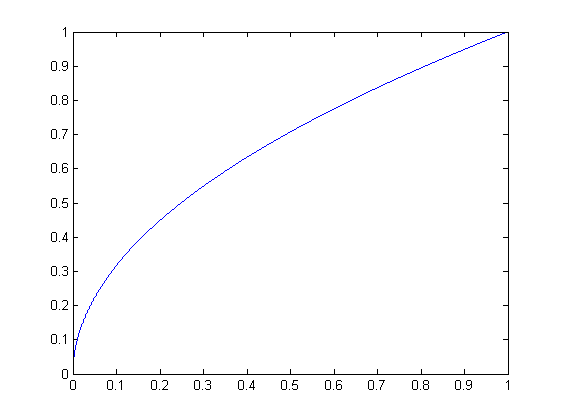
\includegraphics[width=8cm]{bZ}
		\caption{Z}
\end{figure}  

   
   \end {itemize}
\end{description}
\end{document}
